\section{Model predictive control}\label{se:model_predictive_control}
In this section, the design of the controller is elaborated. First the control problem the design of the Model predictive controller (MPC). 

The simulation covered in section ??? is to be controlled with respect to the problems elaborated in section \ref{sec:problem_statement} and stated here. 
\begin{enumerate}
\item Flow variations due to large industries and natural phenomenons
\item Concentration variations due to large industries and natural phenomenons
\begin{enumerate}
	\item Chloride variations
	\item Phosphor variations
	\item Nitrogen variations
	\item Organic matter variations
\end{enumerate}
\end{enumerate}

From the problem statement it is stated that flow and concentration variations must be kept to a minimum without causing any overflow in the sewer. To achieve this tanks are used, these are placed in the sewer network to find locations where they are able to hold back disturbance that will otherwise cause flow and concentration variations into the WWTP. However, the output of these tanks must be controlled in a way where overflow in the tank is prohibited. Therefore the controller must control the output of these tanks in an optimal manner to keep the input variations to the WWTP at a minimum and still be controlled according to some constraints.

To obtain such an optimal behavior MPC is chosen as stated in section \ref{sec:problem_statement}. MPC is an advanced control method which depends on a dynamic model of the system. Where the model, constraints and a cost function is used to generate the most optimal sequence of control inputs to the system, thus obtaining a desired process behavior. However, only the first control input is used in the current timeslot. Hereafter, in the next timeslot, the MPC algorithm is recalculated to find the must optimal input signal for this timeslot and so on. In addition, MPC also take future disturbance into account thereby predicting an output sequence that is optimal including the disturbance.  %The main advantage of MPC  Furthermore, MPC can be used with constraints to calculate the most optimal control output at the given timeslot and taking disturbance into the account. 
% In figure \ref{fig:control_of_sewer} it is shown that the MPC controller is setting the input to the pump.

% \begin{figure}[H]
% \centering
% 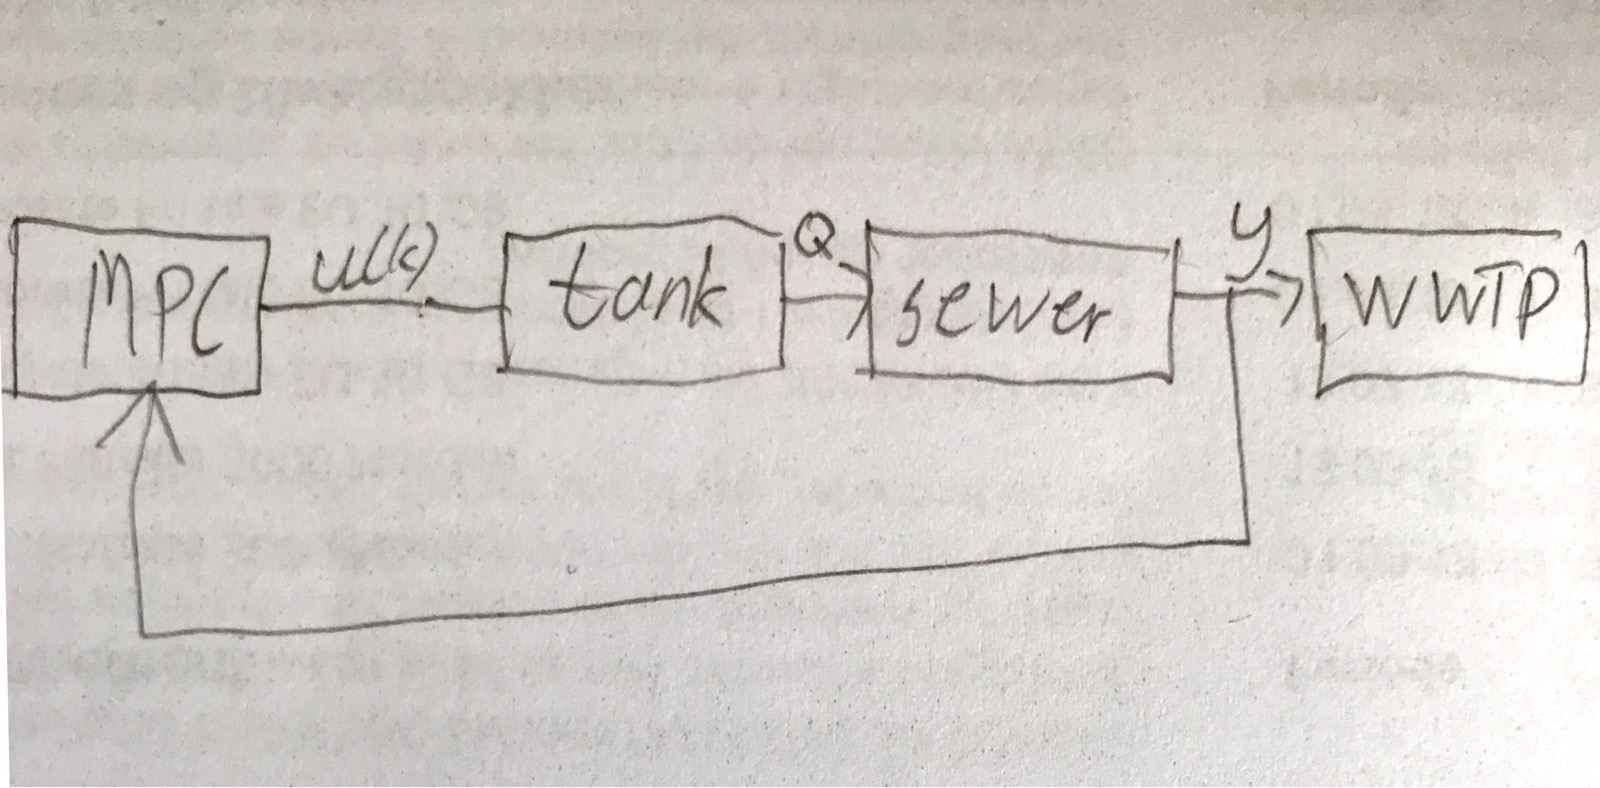
\includegraphics[width=0.8\textwidth]{report/control/pictures/control_of_sewer.jpg}
% \caption{Block diagram of the system.}
% \label{fig:control_of_sewer}
% \end{figure}\fxnote{Der skal staa pumpe i stedet for tank}

% Where the iteration the in the MPC block can be described with the following items. 
% \begin{enumerate}
%        	\item Measurement is taken on the output if possible or it is taken directly from the states. If a state measurement is not available the state is estimated.
%        	\item Calculates a optimal set of predicted values over the prediction horizon according to a cost function and the constraints.
%        	\item The first element of the calculated control sequence is used as the control input.
%        	\item Repeat from 1.
% \end{enumerate}       

For MPC to optimize the system a cost function must be written to penalize variations of the flow output $Q(k+i|k)$ and the concentration output $C(k+i|k)$. Where k defines the time step and i is a value going from $1\leq H_p$, where $H_p$ is the prediction horizon. The cost function for flow and concentration is:

\begin{equation}
	 J = \sum_{i=1}^{H_p-1} || Q(k+i|k)C(k+i|k)-Q(k+i-1|k)C(k+i-1|k)||_{\CMcal{Q}(i)}^2
\end{equation}
Where J is the cost function that needs to be minimized, Q is the flow, C is the concentration and $\CMcal{Q}$ is a weighting parameter. It has been desired to only look at flow variation in the simulation and thereby excluding concentration from the cost function. This has been done to limit the control problem and ease the computation to begin with. Thereby the cost function has been rewritten to: 

\begin{equation}
	 J = \sum_{i=1}^{H_p-1} || \hat{y}(k+i|k)-\hat{y}(k+i-1|k)||_{\CMcal{Q}(i)}^2
\end{equation}
\begin{equation}
	\begin{aligned}
	\text{s.t.} \hspace{5mm}  \hat{x}(k+i+1) &= A\hat{x}(k+i|k)+B\hat{u}(k+i|k)+B\hat{u}_d(k+i|k) \\
						      \hat{y}(k+i)&= C\hat{x}(k+i|k) \\
						     \underline{\hat{x}} \leq \hat{x} \leq \overline{\hat{x}}
	\end{aligned}
\end{equation}
Where Q has been replaced with the output y as it can be measure directly from the state space system. y correspond to the height in the channel, however it is the same to minimize height difference as the flow because both describes the variation in the output of the sewer. 


By using the state equation recursively the variables are collected in extended prediction vectors and matrices denoted by $\CMcal{X,A,B,U,B}_d$ and $\CMcal{U}_d$:


\begin{equation}
\begin{aligned}
	  \underbrace{\begin{bmatrix}
	  \hat{x}(k+1|k) 	\\
	  \hat{x}(k+2|k) 	\\
	  \vdots 			\\
	  \hat{x}(k+H_p|k) 	\\
	   \end{bmatrix}}_{\CMcal{X}}
	 &=
	\underbrace{\begin{bmatrix}
		A \\
		A^2 \\
		\vdots \\
		A^{H_p} \\
	\end{bmatrix}}_{\CMcal{A}}
	x(k) \\&+
	\underbrace{\begin{bmatrix}
		B 		 &0			 &\hdots	& 0		\\
		AB  	 &B  		 & \hdots& 0		\\
		\vdots 	 &\vdots	 & \ddots&\vdots	\\
		A^{H_p-1}B&A^{H_p-2}B&\hdots &B 
    \end{bmatrix}}_{\CMcal{B}}
    	\underbrace{\begin{bmatrix}
	u(k+1|k)\\
	u(k+2|k)\\
	\vdots\\
	u(k+H_p-1|k)
	\end{bmatrix}}_{\CMcal{U}(k)} \\ &+ 
    \underbrace{\begin{bmatrix}
    	B_d 	    &0	         &\hdots & 0		\\
		AB_d  	    &B_d  	     & \hdots& 0		\\
		\vdots 	    &\vdots	     & \ddots&\vdots	\\
		A^{H_p-1}B_d&A^{H_p-2}B_d&\hdots &B_d 
 %   	B & \hdots & 0 \\
 %    	AB+B & \hdots & 0 \\
 %    	\vdots & \ddots & \vdots \\
 %    	\sum_{i=0}^{H_u-1}A^i B & \hdots & B \\
 %    	\sum_{i=0}^{H_u}A^i B & \hdots & AB+B\\
 %    	\vdots & \vdots & \vdots \\
 %    	\sum_{i=0}^{H_p-1}A^i B & \hdots & \sum_{i=0}^{H_p-H_u}A^i B \\
	  \end{bmatrix}}_{\CMcal{B}_d} 
	\underbrace{\begin{bmatrix}
	u_d(k+1|k)\\
	u_d(k+2|k)\\
	\vdots\\
	u_d(k+H_p-1|k)
	\end{bmatrix}}_{\CMcal{U}_d(k)}
	\end{aligned}
\end{equation}






\begin{equation}
	\CMcal{Y}(k)= 
	\begin{bmatrix}
	y(k+1|k)\\
	\vdots\\
	y(k+H_p-1|k)
	\end{bmatrix}
\end{equation}

% \begin{equation}
% 	\Delta U(k)= 
% 	\begin{bmatrix}
% 	\Delta U(k+1|k)\\
% 	\vdots\\
% 	\Delta U(k+H_u -1|k)
% 	\end{bmatrix}
% \end{equation}


\begin{equation}
	\CMcal{C} = diag(C) \hspace{5mm} \psi = \CMcal{C}\CMcal{A}  \hspace{5mm} \gamma = \CMcal{C}\CMcal{B}_u \hspace{5mm}  \Theta = \CMcal{C}\CMcal{B}_{\Delta u}
\end{equation}

\begin{equation}\label{eq:lifted_output_with_states_inserted}
	\CMcal{Y}(k) = \psi x(k) + \gamma \CMcal{U}(k) + \Theta \CMcal{U}_d(k)
\end{equation}





Rewrite cost function to

\begin{equation}
	J = ||\CMcal{Y}(k)-\CMcal{Y}(k-1)||_{Q(i)}^2
\end{equation}

\begin{equation}
	\Delta \CMcal{Y}(k) =\CMcal{Y}(k)-\CMcal{Y}(k-1) 
\end{equation}

Thereby the cost function can be rewritten as:

\begin{equation}\label{eq:delta_cost_function}
	J = \Delta\CMcal{Y}(k)^T \cdot Q \cdot \Delta\CMcal{Y}(k)
\end{equation}

Inserting equation \ref{eq:lifted_output_with_states_inserted} in to equation \ref{eq:delta_cost_function} the follwoing is optained:

\begin{equation}
	J = (\psi\Delta x(k) + \gamma\Delta \CMcal{U}(k) + \Theta\Delta \CMcal{U}_d(k))^T\cdot Q \cdot (\psi\Delta x(k) + \gamma\Delta \CMcal{U}(k) + \Theta\Delta \CMcal{U}_d(k))
\end{equation}

% \begin{equation}
% 	[\CMcal{Y}(k)^T - \CMcal{Y}(k-1)^T]Q[\CMcal{Y}(k) - \CMcal{Y}(k-1)]
% \end{equation}
% \begin{equation}
% 	\CMcal{Y}(k)^TQ\CMcal{Y}(k)+ \CMcal{Y}(k-1)^TQ\CMcal{Y}(k-1)-\CMcal{Y}(k)^TQ\CMcal{Y}(k-1)-\CMcal{Y}(k-1)^TQ\CMcal{Y}(k)
% \end{equation}


By inserting equation ??? into equation ???? only the first term in equation is shown here, the rest can be seen in appendix ????

\begin{equation}
	\begin{aligned}
	&(\psi\Delta x(k) + \gamma\Delta \CMcal{U}(k) + \Theta\Delta \CMcal{U}_d(k))^T\cdot Q \cdot (\psi\Delta x(k) + \gamma\Delta \CMcal{U}(k) + \Theta\Delta \CMcal{U}_d(k)) = \\
	& \Delta x(k)^T\psi ^T Q \psi \Delta x(k) 								+ \underbrace{\Delta x(k)^T \psi ^T Q \gamma}_{Linear} \Delta  \CMcal{U}(k) 				+\Delta x(k)^T \psi ^T Q \Theta \Delta \CMcal{U}_d(k) \\
	& \Delta \CMcal{U}(k)^T \underbrace{\gamma ^T Q \psi\Delta x(k)}_{Linear} + \Delta \CMcal{U}(k)^T\underbrace{\gamma ^T Q \gamma}_{Quadric} \Delta \CMcal{U}(k)+\Delta \CMcal{U}(k)^T \underbrace{\gamma ^T Q\Theta \Delta \CMcal{U}_d(k)}_{Linear} \\ 
	& \Delta \CMcal{U}_d(k)^T \Theta ^T Q  \psi \Delta x(k)					+ \underbrace{\Delta \CMcal{U}_d(k)^T \Theta ^T Q \gamma }_{Linear} \Delta \CMcal{U}(k) 	+\Delta \CMcal{U}_d(k)^T \Theta ^T Q \Theta \Delta \CMcal{U}_d(k)
	\end{aligned}
\end{equation}



\begin{equation}
	\CMcal{H} = \gamma^T Q\gamma 
\end{equation}

\begin{equation}
	\begin{aligned}
	\CMcal{G} &= 2 \Delta x(k)^T\psi^T Q \gamma+2 \Delta \CMcal{U}_d(k)^T\Theta^T Q \gamma 
	\end{aligned}
\end{equation}

And a constant term that can be seen in appendix

\begin{equation}
	J = \Delta U(k)^T\CMcal{H}\Delta U(k)+ \CMcal{G}\Delta U(k)+ c
\end{equation}

The optimization is given by

\begin{equation}
	\min_{\Delta U(k)} J(\Delta U(k)) =\min_{\Delta U(k)} \Delta U(k)^T\CMcal{H}\Delta U(k)+\CMcal{G}\Delta U(k)+c
\end{equation}